\paragraph[QuizziPedia::Front-End::ModelViews\\::ResultsQuestionnaireModelView]{QuizziPedia::Front-End::ModelViews::ResultsQuestionnaireModelView}
	
	\label{QuizziPedia::Front-End::ModelViews::ResultsQuestionnaireModelView}
	
	\begin{figure}[ht]
		\centering
		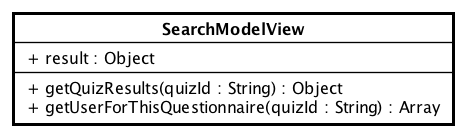
\includegraphics[scale=0.8,keepaspectratio]{UML/Classi/Front-End/QuizziPedia_Front-end_ModelView_ResultsQuestionnaireModelView.png}
		\caption{QuizziPedia::Front-End::ModelViews::ResultsQuestionnaireModelView}
	\end{figure} \FloatBarrier
	
	\begin{itemize}
		\item \textbf{Descrizione}: classe di tipo modelview la cui istanziazione è contenuta all'interno della variabile di ambiente \texttt{\$scope} di \textit{Angular\ped{G}}. All'interno di essa sono presenti le variabili e i metodi necessari per il \textit{Two-Way Data-Binding\ped{G}} tra la \textit{view\ped{G}} \texttt{ResultsQuestionnaireView} e il \textit{controller\ped{G}} \texttt{ResultsQuestionnaireController};
		\item \textbf{Utilizzo}: viene utilizzata per effettuare il \textit{Two-Way Data-Binding\ped{G}} tra la \textit{view\ped{G}}\\ \texttt{ResultsQuestionnaireView} e il \textit{controller\ped{G}} \texttt{ResultQuestionnaireController} rendendo disponibili variabili e metodi;
		\item \textbf{Relazioni con altre classi}: 
		\begin{itemize}
			\item \textbf{OUT \texttt{ResultsQuestionnaireView}}: \textit{view\ped{G}} contenente i risultati conseguiti dagli utenti che hanno compilato il proprio questionario; 
			\item \textbf{OUT \texttt{ResultQuestionnaireController}}: questa classe permette di gestire la ricerca di questionari e utenti all’interno dell’applicazione;
		\end{itemize}
		\item \textbf{Attributi}: 
		\begin{itemize}
				\item \texttt{+ results: Object} \\ \texttt{array} contenente un oggetto per ogni iscritto che ha compilato il questionario. L'oggetto sarà composto dai campi: \texttt{nome} e \texttt{cognome} e \texttt{valutazione}.
		\end{itemize}
		\item \textbf{Metodi}: 
		\begin{itemize}
			\item \texttt{+ getQuizResults(quizId: String): Object} \\ Metodo che ritorna i risultati di un questionario.\\
			\textbf{Parametri}:
			\begin{itemize}
				\item \texttt{quiId: String} \\ 
				Id del questionario del quale recuperare i risultati.
			\end{itemize}
			\item \texttt{+ getUserForThisQuestionnaire(quizId: String): Array} \\ Metodo che ritorna tutti gli utenti che hanno eseguito il questionario, con il loro risultato.\\
			\textbf{Parametri}:
			\begin{itemize}
				\item \texttt{quizId: String} \\ Id del questionario del quale recuperare gli utenti.
			\end{itemize}
				
		\end{itemize}
	\end{itemize}

	